\section{VM-centric Snapshot Deduplication}
\label{sect:deduplication}

%\subsection{VM centric  strategies}
%\label{sect:vc-strategies}

We describe our overall deduplication approach as consisting of three
complementary strategies: VM-local
duplicate search optimization, global deduplication using popular chunks, and 
VM-centric file system block management. 
%\begin{itemize}
%\item 

\textbf{VM-local duplicate search optimization} --
We use the standard version-based detection~\cite{Clements2009,Vrable2009}
to identify changed content with dirty bits in a coarse grain segment level.
%In our implementation 
%the segment size is 2MB
%and the device driver is extended to support tracking changed segments using a dirty bitmap. 
The reason to choose a coarse grain level is that 
since every write for a segment will touch a dirty bit, the device driver maintains dirty bits in 
memory and cannot afford a small segment size.
It should be noted that dirty bit tracking is supported or can be easily implemented in 
major virtualization solution vendors. 
%% this method is so widely-used and easy to understand, everyone include Pure Storage has it, I feel no need to explain further.
%{
%For example,
%the VMWare hypervisor has an API to let external backup applications know 
%the changed areas since last backup. 
%The Microsoft SDK provides an API that allows external applications to monitor 
%the VM's I/O traffic and implement such changed block tracking feature.
%}

\begin{figure}[htbp]
  \centering
  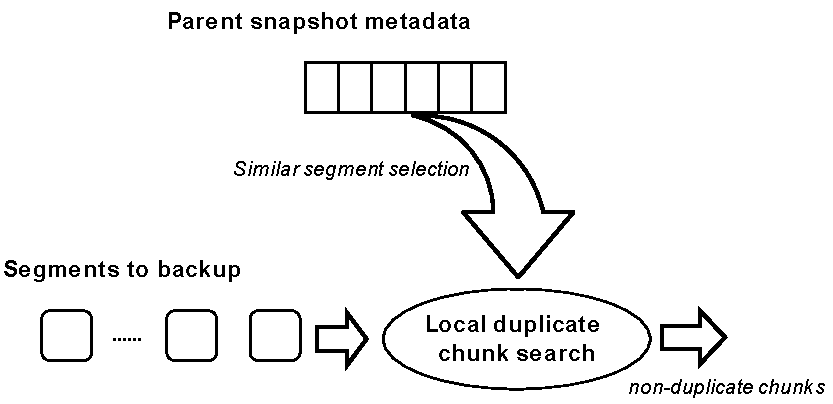
\epsfig{file=images/mh_local_dedup.pdf, width=3in}
  \caption{Similarity-guided local duplicate detection}
  \label{fig:local_dedup}
\end{figure}

Since the best deduplication uses a non-uniform chunk size 
with an average of 4KB or 8KB~\cite{Jin2009},
we conduct additional local similarity guided deduplication on a snapshot by comparing
chunk fingerprints of a dirty segment 
with those in  {\em similar} segments from its parent snapshot. 
We define two segments are similar if their content signature is the same.
This segment content signature value is defined as the minimum value of all its chunk fingerprints 
computed during backup and is recorded in the snapshot metadata (called recipe). Note that this definition of
content similarity is an approximation~\cite{resemblance97}.  When processing a dirty segment,
its  similar segments can be found easily from the
parent snapshot recipe.  Then recipes of the similar segments are loaded to memory,
which contain chunk fingerprints to be compared.
To control the time cost of search, we set a limit on the number of  similar segment recipes to be fetched. 
% Then,
%given a set of data chunks within a dirty segment,  we compare  these chunk fingerprints
%with those in similar segments.  
For example, assume that  a segment is of size  2MB, 
its segment recipe is roughly 19KB which contains about 500 chunk fingerprints and other chunk metadata.
By limiting at most 10 similar segments to search, the amount of memory for maintaining those 
similar segment recipes is small.
As part of our local duplicate search we also compare the current segment
against the parent segment at the same offset.

%\item 
\textbf{Global deduplication using popular chunks} --
This step accomplishes the canonical global fingerprint lookup using a popular fingerprint index.
Our key observation is that the local deduplication has removed most of the duplicates.
There are fewer deduplication opportunities across VMs while the memory and network
consumption for global comparison is more expensive.
Thus our approximation is that the global fingerprint comparison only searches for the top $k$
most popular items. This dataset is called the \textbf{PDS} (popular data set). 
We define chunk popularity as the number of unique copies of the chunk in the data-store,
i.e., the number of copies of the chunk after local deduplication.
This number can be computed periodically, e.g., on a weekly basis.
Once the popularity of all data chunks is collected, the system only maintains the top $k$
most popular chunk fingerprints (called \textbf{PDS index}) in a distributed shared memory.  
%Compared to a preliminary solution which  uses data popularity~\cite{WeiZhangIEEE}, 
%this paper provides  a more comprehensive scheme with  improved deduplication efficiency and fault tolerance, and
%analytic design guidance. 

Since $k$ is relatively small and these top $k$ chunks are shared among multiple VMs, 
we can afford to provide extra replicas for these popular chunk data to enhance the fault resilience.
We have studied the distribution of chunk popularity~\cite{WeiZhangIEEE} 
based on a data trace from Alibaba with over 2500 VMs.
The distribution is zipf-like and popular chunks dominate the distribution.
We denote $\sigma$ as the percentage of unique data chunks belonging to PDS and from the evaluation we find that
$\sigma$ with a range of 1 to 4\% can deliver a fairly competitive deduplication efficiency.

% Figure~\ref{fig:Datazipf} illustrates the distribution of chunk popularity based on a data trace from Alibaba with over 2500 VMs.
% The distribution is zipf like and popular chunks are dominating the large portion of data chunks.
% We denote $\sigma$ as the percentage of unique data chunks belonging to PDS and from the evaluation we find that
% $\sigma$ with a range of 1 to 4\% can deliver a fairly competitive deduplication efficiency.

%\item 
\textbf{VM-centric file system block management} --
When a chunk is not detected as a duplicate to any existing chunk, this chunk will be written
to the file system. Since the backend file system typically uses a large block size such as 64MB, each VM will 
accumulate small local chunks. We manage this accumulation process using a log-structured storage scheme built
on a distributed file system discussed in Section~\ref{sect:architecture}.
%Non-PDS chunks from the same VM are stored in one append store. 
Each file system block is either dedicated to non-PDS chunks, or PDS-chunks.
A file system block for non-PDS chunks is associated with one VM and does not contain
any PDS chunks, such that our goal of fault isolation is maintained.
In addition, storing PDS chunks separately allows special replication handling for those popular shared data. 
%%% talk something about snapshot store advantage here? %%%


%One could try to rely on filesystem features to 
If we do not separate the
popular chunks from the less-popular, the popular chunks are dispersed across
all of the filesystem blocks in the storage system.  Then we cannot leverage the file system features to 
provide extra replication to popular and shared chunks because  
we have to add extra replication to each file block as long as it contains a popular chunk.

%factor on popular chunks. This explains why we must separate the PDS and
%non-PDS data in our system to achieve the desired $r_c/r$ ratio (though both
%can be stored on the same DFS).

%The system allows all machines conduct backups in parallel, and each machine
%conducts the backup of one VM at a time, and thus only requires a write buffer for one VM.
%\end{itemize}

% \begin{figure}
% \centering
%  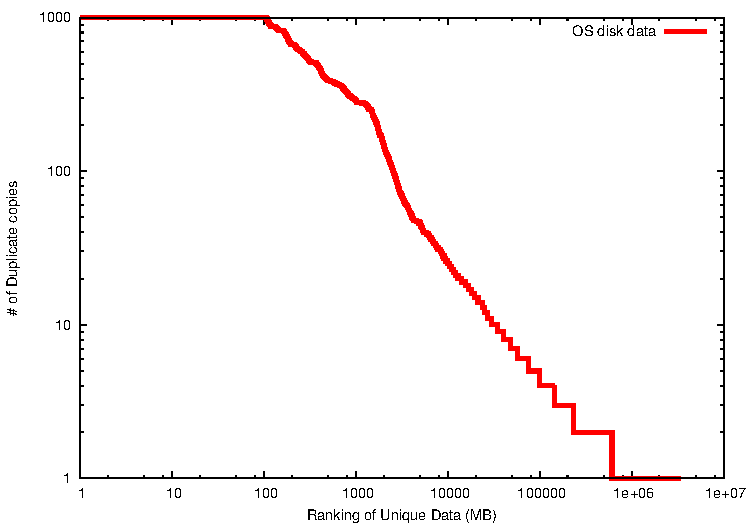
\includegraphics[width=3in]{figures/log-log-disk}
% \caption{Duplicate frequency versus  chunk ranking in a log scale after local deduplication.}
% \label{fig:Datazipf}
% \end{figure}


% {\it [Need to find a place to put these numbers in: Total number of chunks 
% in 350 snapshots: 1,546,635,485. 
% Total number of chunks after localized dedup: 283,121,924. Total number of unique chunks: 87,692,682.]}

